En una actividad del colegio Comfaboy, se diseña una figura compuesta para un mural. La figura está formada por:

- Un rectángulo de 9 m de largo y 4,5 m de alto  
- Un triángulo isósceles unido al lado izquierdo, con base igual a la altura del rectángulo (4,5 m) y una profundidad de 3,5 m  
- Un semicírculo unido al lado derecho del rectángulo, cuyo diámetro es 4,5 m  

\begin{center}
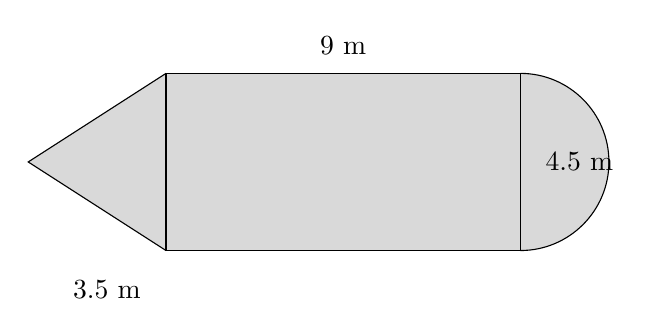
\begin{tikzpicture}[scale=0.5]

% Rectángulo sombreado
\fill[gray!30] (0,0) rectangle (9,4.5);

% Triángulo sombreado
\fill[gray!30] (0,0) -- (-3.5,2.25) -- (0,4.5) -- cycle;

% Semicírculo sombreado (correcto)
\fill[gray!30]
(9,0) -- (9,4.5)
arc[start angle=90,end angle=-90,radius=2.25] -- cycle;

% Bordes
\draw (0,0) rectangle (9,4.5);
\draw (0,0) -- (-3.5,2.25) -- (0,4.5);
\draw (9,0) arc[start angle=-90,end angle=90,radius=2.25];

% Medidas
\node at (4.5,5.2) {9 m};
\node at (-1.5,-1) {3.5 m};
\node at (10.5,2.25) {4.5 m};

\end{tikzpicture}
\end{center}

¿Cuál es el área total de la figura?

\begin{multicols}{2}
\begin{enumerate}[label=\alph*), leftmargin=*]
\item $40.5 + 7.875 + \frac{1}{2}\pi(2.25)^2$
\item $40.5 + 15.75 + \pi(2.25)^2$
\item $40.5 + 7.875 + \pi(2.25)^2$
\item $40.5 + 7.875$
\end{enumerate}
\end{multicols}